\documentclass[10pt,conference]{IEEEtran}
\IEEEoverridecommandlockouts

\usepackage[utf8]{inputenc}
\usepackage[T1]{fontenc}
\usepackage{cite}
\usepackage{amsmath,amssymb}
\usepackage{graphicx}
\usepackage{booktabs}
\usepackage{url}
\usepackage{xspace}
\usepackage{xcolor}
\usepackage{balance}
\usepackage{tikz}
\usetikzlibrary{positioning,arrows.meta}

% Gerado por src/fase6_paper.py a partir de results/ e data/derived/. Não editar à mão.
\newcommand{\Seed}{20270402\xspace}
\newcommand{\NScanned}{89,649\xspace}
\newcommand{\NDomain}{28,244\xspace}
\newcommand{\NDomainStrong}{27,736\xspace}
\newcommand{\NDomainWeak}{508\xspace}
\newcommand{\NStrongTerms}{75\xspace}
\newcommand{\NWeakTerms}{17\xspace}
\newcommand{\NTestTerms}{56\xspace}
\newcommand{\NPool}{4,928\xspace}
\newcommand{\NPoolRepos}{2,100\xspace}
\newcommand{\NPoolCopies}{12,314\xspace}
\newcommand{\NPoolWithCopies}{1,073\xspace}
\newcommand{\NPoolMaxCopies}{302\xspace}
\newcommand{\NGroups}{3,314\xspace}
\newcommand{\NInGroups}{2,078\xspace}
\newcommand{\PctInGroups}{42.2\%\xspace}
\newcommand{\NMaxGroup}{151\xspace}
\newcommand{\NMain}{384\xspace}
\newcommand{\NCal}{30\xspace}
\newcommand{\NSub}{60\xspace}
\newcommand{\NTrunc}{246\xspace}
\newcommand{\PctTrunc}{64.1\%\xspace}
\newcommand{\NPerm}{128\xspace}
\newcommand{\NBands}{16\xspace}
\newcommand{\NShingle}{5\xspace}
\newcommand{\JaccardMin}{0.8\xspace}
\newcommand{\NBigGroupSkills}{625\xspace}
\newcommand{\PctBigGroupSkills}{12.7\%\xspace}
\newcommand{\PctSingletons}{57.8\%\xspace}
\newcommand{\LexPoolQone}{23.7\%\xspace}
\newcommand{\LexSampleQone}{24.5\%\xspace}
\newcommand{\LexPoolQtwo}{18.5\%\xspace}
\newcommand{\LexSampleQtwo}{19.5\%\xspace}
\newcommand{\LexPoolQthree}{5.1\%\xspace}
\newcommand{\LexSampleQthree}{3.6\%\xspace}
\newcommand{\LexPoolQfour}{12.8\%\xspace}
\newcommand{\LexSampleQfour}{11.7\%\xspace}
\newcommand{\LexPoolQfive}{20.8\%\xspace}
\newcommand{\LexSampleQfive}{15.6\%\xspace}
\newcommand{\LexPoolQsix}{3.0\%\xspace}
\newcommand{\LexSampleQsix}{3.1\%\xspace}
\newcommand{\LexPoolQseven}{0.1\%\xspace}
\newcommand{\LexSampleQseven}{0.3\%\xspace}
\newcommand{\LexPoolQeight}{35.7\%\xspace}
\newcommand{\LexSampleQeight}{36.5\%\xspace}
\newcommand{\LexPoolQnine}{32.1\%\xspace}
\newcommand{\LexSampleQnine}{29.4\%\xspace}
  % gerado por src/fase6_paper.py — todo número vem de results/*.json
\newcommand{\todo}[1]{\textcolor{red}{[TODO: #1]}}

\begin{document}

\title{What Testing Practices Do Blockchain Agent Skills Instruct?\\
A Testing Skill Profile of GitSkills}

% Double-anonymous submission: no author block.
\author{\IEEEauthorblockN{Anonymous Author(s)}}

\maketitle

\begin{abstract}
\todo{abstract (deadline 18 Dec 2026)}
\end{abstract}

\begin{IEEEkeywords}
Agent Skills, Software Testing, Test Pyramid, Blockchain-Oriented Software Engineering, Mining Software Repositories
\end{IEEEkeywords}

%% ---------------------------------------------------------------------------
\section{Introduction}
\label{sec:intro}

\todo{motivation: agent skills instruct coding agents in natural language, with no compiler checking their testing guidance; in blockchain, faults in value-bearing code are costly and irreversible.}

We investigate which testing practices the agent skills of the blockchain domain instruct the agent to follow, using the Practical Test Pyramid~\cite{vocke2018pyramid} as reference. We address two research questions:

\textbf{RQ1 (Profile).} Which test layers do the skills instruct, and in which context (on-chain, off-chain Web3, Web2)?

\textbf{RQ2 (Practices).} Which good and bad testing practices do the skills instruct, and how often per category and context?

\todo{contributions C1--C3: Testing Skill Profile; catalog of practices with quotes; reusable instrument and annotations.}

%% ---------------------------------------------------------------------------
\section{Methodology}
\label{sec:method}

Our methodology follows a Mining Software Repositories (MSR) approach structured in six phases, as shown in Figure~\ref{fig:method}. The unit of analysis is one distinct \texttt{SKILL.md} file. All scripts use a fixed seed (\Seed), every execution is logged, and every number reported in this paper is read from a file generated by a script, available in the replication package~\cite{replication}.

% Figura 1 — metodologia em seis fases. Números vêm de numeros.tex (gerado de results/*.json).
\begin{figure*}[t]
\centering
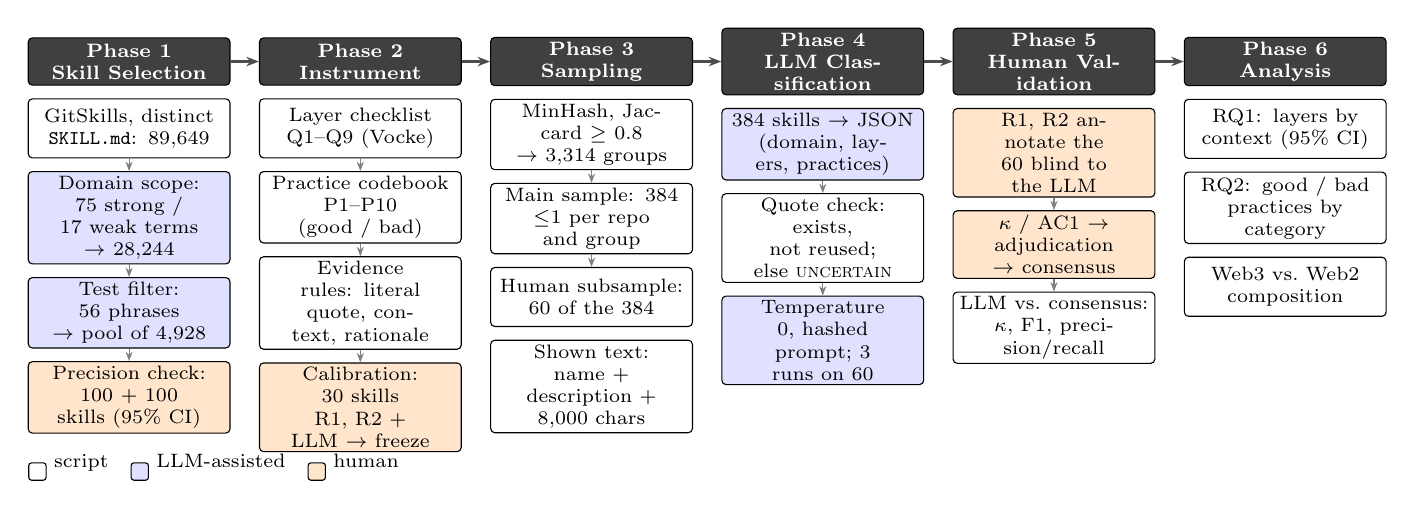
\begin{tikzpicture}[
  font=\scriptsize, node distance=1.6mm and 3.6mm,
  base/.style={draw, rounded corners=1.5pt, align=center, text width=24.5mm, minimum height=7.5mm, inner sep=1.6pt},
  phase/.style={base, fill=black!75, text=white, font=\scriptsize\bfseries, minimum height=6mm},
  auto/.style={base, fill=white},
  llm/.style={base, fill=blue!12},
  human/.style={base, fill=orange!20},
  arr/.style={-{Stealth[length=1.6mm]}, thick, black!70},
  link/.style={-{Stealth[length=1.2mm]}, black!50},
]
% ---- Phase headers
\node[phase] (h1) {Phase 1\\Skill Selection};
\node[phase, right=of h1] (h2) {Phase 2\\Instrument};
\node[phase, right=of h2] (h3) {Phase 3\\Sampling};
\node[phase, right=of h3] (h4) {Phase 4\\LLM Classification};
\node[phase, right=of h4] (h5) {Phase 5\\Human Validation};
\node[phase, right=of h5] (h6) {Phase 6\\Analysis};
\foreach \a/\b in {h1/h2, h2/h3, h3/h4, h4/h5, h5/h6} \draw[arr] (\a) -- (\b);

% ---- Phase 1
\node[auto, below=of h1] (p1a) {GitSkills, distinct\\\texttt{SKILL.md}: \NScanned};
\node[llm, below=of p1a] (p1b) {Domain scope: \NStrongTerms strong /\\\NWeakTerms weak terms $\rightarrow$ \NDomain};
\node[llm, below=of p1b] (p1c) {Test filter: \NTestTerms phrases\\$\rightarrow$ pool of \NPool};
\node[human, below=of p1c] (p1d) {Precision check:\\100 + 100 skills (95\% CI)};
\foreach \a/\b in {p1a/p1b, p1b/p1c, p1c/p1d} \draw[link] (\a) -- (\b);

% ---- Phase 2
\node[auto, below=of h2] (p2a) {Layer checklist\\Q1--Q9 (Vocke)};
\node[auto, below=of p2a] (p2b) {Practice codebook\\P1--P10 (good / bad)};
\node[auto, below=of p2b] (p2c) {Evidence rules: literal\\quote, context, rationale};
\node[human, below=of p2c] (p2d) {Calibration: \NCal skills\\R1, R2 + LLM $\rightarrow$ freeze};
\foreach \a/\b in {p2a/p2b, p2b/p2c, p2c/p2d} \draw[link] (\a) -- (\b);

% ---- Phase 3
\node[auto, below=of h3] (p3a) {MinHash, Jaccard $\geq$ \JaccardMin\\$\rightarrow$ \NGroups groups};
\node[auto, below=of p3a] (p3b) {Main sample: \NMain\\$\leq$1 per repo and group};
\node[auto, below=of p3b] (p3c) {Human subsample:\\\NSub of the \NMain};
\node[auto, below=of p3c] (p3d) {Shown text: name +\\description + 8,000 chars};
\foreach \a/\b in {p3a/p3b, p3b/p3c} \draw[link] (\a) -- (\b);

% ---- Phase 4
\node[llm, below=of h4] (p4a) {\NMain skills $\rightarrow$ JSON\\(domain, layers, practices)};
\node[auto, below=of p4a] (p4b) {Quote check: exists,\\not reused; else \textsc{uncertain}};
\node[llm, below=of p4b] (p4c) {Temperature 0, hashed\\prompt; 3 runs on \NSub};
\foreach \a/\b in {p4a/p4b, p4b/p4c} \draw[link] (\a) -- (\b);

% ---- Phase 5
\node[human, below=of h5] (p5a) {R1, R2 annotate the\\\NSub blind to the LLM};
\node[human, below=of p5a] (p5b) {$\kappa$ / AC1 $\rightarrow$\\adjudication $\rightarrow$ consensus};
\node[auto, below=of p5b] (p5c) {LLM vs.\ consensus:\\$\kappa$, F1, precision/recall};
\foreach \a/\b in {p5a/p5b, p5b/p5c} \draw[link] (\a) -- (\b);

% ---- Phase 6
\node[auto, below=of h6] (p6a) {RQ1: layers by\\context (95\% CI)};
\node[auto, below=of p6a] (p6b) {RQ2: good / bad\\practices by category};
\node[auto, below=of p6b] (p6c) {Web3 vs.\ Web2\\composition};

% ---- Legend
\node[anchor=north west, inner sep=0pt] at ([yshift=-2.5mm]p1d.south west) {%
  \tikz[baseline=-0.6ex]\node[draw, rounded corners=1pt, fill=white, minimum size=2.2mm]{}; script\quad
  \tikz[baseline=-0.6ex]\node[draw, rounded corners=1pt, fill=blue!12, minimum size=2.2mm]{}; LLM-assisted\quad
  \tikz[baseline=-0.6ex]\node[draw, rounded corners=1pt, fill=orange!20, minimum size=2.2mm]{}; human};
\end{tikzpicture}
\caption{Methodology in six phases. Numbers are those of the current execution (seed \Seed).}
\label{fig:method}
\end{figure*}


\subsection{Phase 1: Skill Selection}
\label{sec:selection}

Related to the \textbf{Data Source}, we use GitSkills~\cite{gitskills2027}, a snapshot of the \texttt{SKILL.md} files publicly visible on GitHub in July 2026, with 1,877,981 distinct contents from 282,200 repositories. GitSkills groups verbatim copies by content hash and marks one representative per group (\texttt{dedup\_primary}~$=1$), which we use to avoid counting the same text more than once. We start from the subset of \NScanned distinct skills that match at least one term of a broad blockchain vocabulary. \todo{re-run Phase 1 on the full 41\,GB database and update this sentence.}

In \textbf{Domain Scoping}, we restrict this subset to the blockchain domain with a vocabulary split into two classes. \textit{Strong} terms are sufficient on their own (e.g., ``solidity'', ``smart contract'', ``hardhat'', ``forge test''), while \textit{weak} terms are ambiguous outside the domain and only count when two distinct weak terms co-occur or when a strong term is present (e.g., ``wallet'', ``gas'', ``token address''). The terms were proposed by an LLM and reviewed by two researchers, resulting in \NStrongTerms strong and \NWeakTerms weak terms. We match them as case-insensitive patterns delimited by non-alphanumeric characters, applied to the name, description, and content of each skill. We adopted this split because a first version, in which weak terms were generic words in LLM-oriented skills (e.g., ``tokens'', ``layer~1'', ``validators''), admitted mostly Web2 skills such as planning and review workflows. Unambiguous forms were kept as strong (e.g., ``foundry.toml'' rather than ``foundry'', which also names cloud AI platforms), and generic forms were removed or qualified. The domain scope comprises \NDomain skills, of which \NDomainStrong contain a strong term and \NDomainWeak entered through weak terms only.

In \textbf{Test Filtering}, we keep the skills that contain at least one of \NTestTerms compound testing phrases, generated and reviewed in the same way (e.g., ``unit test'', ``forge test'', ``fuzz'', ``invariant test'', ``playwright''). We never use the isolated word ``test'', which occurs in many skills that do not address testing. This filter only selects candidates; the classification itself is carried out in Phases~4 and~5. The resulting pool has \NPool skills from \NPoolRepos repositories. Since \NPoolWithCopies of these contents have verbatim copies (up to \NPoolMaxCopies each), the pool corresponds to \NPoolCopies file occurrences in GitSkills.

In \textbf{Selection Validation}, one researcher checks 100 skills randomly drawn from the domain scope (``is this skill about blockchain/Web3?'') and 100 from the pool (``does this skill address testing?''), blind to the matched terms. We report the precision of each step with a 95\% Wilson confidence interval~\cite{wilson1927}, with a target of at least 0.90. Precision was \todo{domain: $p$ [CI]; test: $p$ [CI]}.

\subsection{Phase 2: Instrument}
\label{sec:instrument}

The same text serves as the human guideline and as the LLM prompt, so that both apply identical criteria. Each item is answered with a single question: \textit{does the text instruct the agent to do this?} Mentioning or listing a practice does not count.

\textbf{Context and domain class.} Each piece of evidence receives a context defined by what the tested component does, not by the repository where it lives: \textit{on-chain} (code executed by the blockchain, e.g., Solidity, Vyper or Anchor programs, proxies, deploy scripts), \textit{off-chain Web3} (code outside the chain that reads or writes chain state, signs transactions, manages keys, or consumes ABIs and events, e.g., dApps with a wallet, SDK/RPC clients, indexers, bots, bridges), or \textit{Web2} (code with no chain interaction, even inside a Web3 project). Each skill also receives a domain class: \texttt{onchain}, \texttt{offchain\_web3}, \texttt{mixed}, \texttt{web2\_incidental} (blockchain is a peripheral mention), or \texttt{undetermined}. This class answers whether the skills in our scope are predominantly Web3 or Web2.

\textbf{Layer checklist.} Nine items cover the layers of the Practical Test Pyramid~\cite{vocke2018pyramid}: Q1~Unit, Q2~Integration, Q3~Contract, Q4~UI, Q5~End-to-End, Q6~Acceptance, Q7~Exploratory, and Q8~Automation, plus Q9~Web3-specific techniques (fork, fuzz, invariant, formal verification, and gas testing). The YES criterion of each item paraphrases the corresponding section of Vocke~\cite{vocke2018pyramid}, and its adaptation to blockchain follows the Foundry, Hardhat, and Anchor documentation~\cite{foundrybook,hardhatdocs,anchordocs}. For example, Q1 is YES when the skill instructs testing a contract function with mocked dependencies, or an SDK function with a stubbed RPC; ``run the tests'' alone does not count. Similarly, Q2 requires a real junction (contract to contract on a local chain, or backend to RPC node), and a mainnet fork without checking the junction does not count.

\textbf{Practice codebook.} Ten categories capture good and bad testing practices: P1~pyramid balance, P2~isolation, P3~assertions, P4~determinism, P5~adversarial testing, P6~automation and CI, P7~coverage, P8~test integrity, P9~secrets, and P10~other practices emerging in calibration. Polarity is anchored in sources rather than in the annotator's opinion: Vocke~\cite{vocke2018pyramid}, the test smells catalog of Garousi and K\"u\c{c}\"uk~\cite{garousi2018smells}, the Foundry Book~\cite{foundrybook}, the ConsenSys Smart Contract Best Practices~\cite{consensys}, and the OWASP Smart Contract Top~10~\cite{owaspsc}. For instance, pinning a fork to a block number is a good P4 practice, whereas a fork without a pinned block is a bad one; fixing the code is a good P8 practice, whereas skipping or loosening a failing test is a bad one.

\textbf{Evidence rules.} Each YES and each practice requires a literal quote of 5 to 40 words and a one-sentence justification linking the quote to the criterion or category, together with its context. Only what is instructed counts, and a quote cannot justify two different items. In \textbf{Calibration}, two researchers and the LLM annotate \NCal skills outside the sample, adjust the examples once (including new P10 categories), and freeze the instrument. \todo{calibration outcome: changes and new P10 categories.}

\subsection{Phase 3: Sampling}
\label{sec:sampling}

GitSkills reports that 50.5\% of all file occurrences are verbatim copies~\cite{gitskills2027}, and templates are also copied with small edits. To prevent a single template from dominating the sample, we group \textbf{near-duplicates} with MinHash~\cite{broder1997} (\NPerm permutations over \NShingle-word shingles, locality-sensitive hashing with \NBands bands) and link two skills when their estimated Jaccard similarity is at least \JaccardMin. The pool forms \NGroups groups, and \NInGroups skills (\PctInGroups) belong to a group with two or more members; the largest group has \NMaxGroup machine-generated skills sharing the same boilerplate. Figure~\ref{fig:groups} shows that only \PctSingletons of the pool skills are unique, and \PctBigGroupSkills belong to templates with more than 20 variants, which would otherwise dominate any random sample.

\begin{figure}[t]
\centering
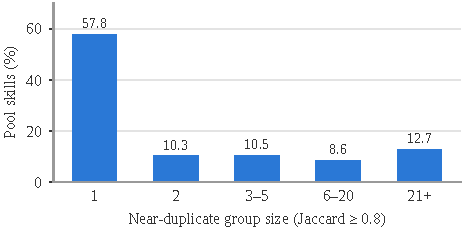
\includegraphics[width=\columnwidth]{figures/grupos_tamanho.pdf}
\caption{Share of the \NPool pool skills by the size of their near-duplicate group. \PctSingletons are unique, while \PctBigGroupSkills belong to templates with more than 20 variants.}
\label{fig:groups}
\end{figure}

For the \textbf{Main Sample}, we draw \NMain skills from the pool, which gives a 95\% confidence level with a $\pm$5\% margin~\cite{cochran1977}. We shuffle the pool with the fixed seed and accept a skill only if neither its repository nor its near-duplicate group has been selected, so the sample holds at most one skill per repository and per group. The \NCal calibration skills are drawn next under the same constraints, so they share no repository or group with the main sample. A \textbf{Human Subsample} of \NSub skills is drawn within the \NMain. The text shown to the LLM and to the annotators is identical: name, description, and content up to 8,000 characters; \NTrunc skills (\PctTrunc) of the main sample exceed this limit and are truncated.

Figure~\ref{fig:lexical} compares the pool and the main sample on lexical testing signals, i.e., the test phrases of Phase~1 mapped to the checklist layers. The pool value falls within the 95\% confidence interval of the sample for eight of the nine layers. The exception is E2E (\LexPoolQfive in the pool versus \LexSampleQfive in the sample), because a single end-to-end testing template copied across dozens of repositories inflates the pool and is represented only once in the sample. These signals only describe the candidates; whether the skills actually \textit{instruct} each layer is decided in Phases~4 and~5.

\begin{figure}[t]
\centering
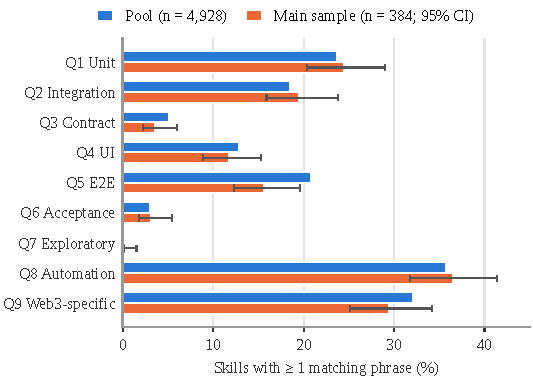
\includegraphics[width=\columnwidth]{figures/camadas_lexicas.pdf}
\caption{Lexical testing signals per checklist layer: share of skills whose text contains at least one test phrase mapped to the layer. These are term matches used for candidate selection, not the classification of Phases~4--5 (e.g., ``contract testing'' also matches ``smart contract testing'').}
\label{fig:lexical}
\end{figure}

\subsection{Phase 4: LLM Classification}
\label{sec:llm}

The LLM\footnote{\todo{exact model and version.}} classifies each of the \NMain skills and returns a JSON object with the domain class; the answer, quote, justification, and context for Q1--Q9; and a list of practices, each with quote, category, polarity, context, and justification. An \textbf{Automatic Check} verifies that every quote exists in the shown text and is not reused across items; an item that fails twice becomes \textsc{uncertain} and is counted as discarded. We use temperature 0, record the SHA-256 hash of the prompt, and run the \NSub skills of the subsample three times to measure the stability of the answers. \todo{discard rate; stability across the three runs.}

\subsection{Phase 5: Human Annotation and Validation}
\label{sec:human}

In \textbf{Blind Annotation}, two researchers (R1 and R2) independently annotate the \NSub skills of the subsample without seeing the LLM output, using per-annotator sheets in which skills are identified only by an opaque ID. We measure \textbf{Human Agreement} with Cohen's $\kappa$~\cite{cohen1960} per item, and Gwet's AC1~\cite{gwet2008} for rare items, where $\kappa$ is unstable; disagreements are then adjudicated into a consensus. To compare the \textbf{LLM with the Consensus}, we compute $\kappa$ and F1 per layer, per context, and per domain class. For practices, we compute precision and recall, matching quotes that overlap by at least 50\%, and $\kappa$ for category and polarity. Any item in which the LLM reaches $\kappa < 0.40$ is reported with the human values only. \todo{agreement values (Tab.~II).}

\subsection{Phase 6: Analysis}
\label{sec:analysis}

For RQ1, we report the percentage of skills with YES per layer, with 95\% confidence intervals, split by context, and the Web3 versus Web2 composition of the scope. For RQ2, we count good and bad practices per category and context, with a short example of each polarity.

%% ---------------------------------------------------------------------------
\section{Results}
\label{sec:results}
\todo{RQ1: Fig.~2 (profile by context). RQ2: Tab.~I (catalog of practices).}

\section{Discussion}
\label{sec:discussion}
\todo{}

\section{Threats to Validity}
\label{sec:threats}
\todo{term-based selection (precision measured in Phase 1); subset of GitSkills rather than the full snapshot; LLM over-classification (consensus as reference, mandatory quotes, automatic check); subjective polarity (anchored in sources, agreement measured); on/off-chain/Web2 boundary (explicit decision rule, $\kappa$ reported); truncation of \PctTrunc of the sample at 8,000 characters; instruction is not actual practice; copies (deduplication and one skill per repository and group).}

\section{Ethics}
\label{sec:ethics}
\todo{mandatory section: public data, no personal data, anonymised authors in GitSkills, annotation by the authors only.}

\section{Conclusion and Data Availability}
\label{sec:conclusion}
\todo{} The checklist, codebook, prompt, scripts, and annotations are available in an anonymized repository~\cite{replication}.

\balance
\bibliographystyle{IEEEtran}
\bibliography{references}

\end{document}
